\subsubsection{Server Structure}
When setting up the server side, the project was divided into different blocks. Each block has its own responsibility as far as possible. If done correctly there are many benefits by splitting code into different blocks. The standard way of splitting code is to follow SOLID (S: Single responsibility principle, O: Open–closed principle, L: Liskov substitution principle, I: Interface segregation principle, D: Dependency inversion principle). If this is followed correctly it gives the advantages of MURDER (M: Maintainability, U: Understandability, R: Reusability, D: Debugability, E: Extensibility, R: Regression). Examples of this can be seen in how the socket functions are split up into categories. Client functions, admin functions, and Feide functions are split into their own file and then imported where they are needed. The same can be seen in the database functions, where get, insert, update and delete functions are split into their own files to make development easier. When it comes to extensibility, the server is written to be able to scale up with more question types in a straightforward manner. The way the server handles generating a solution, validating a question and checking an answer is written into their own files based on the question type. This makes it so that if another question type is added, the developer only need to add a couple of lines in each master file to make it work. The developer also needs to implement their algorithms in separate files.
\begin{figure}[H]
    \centering
    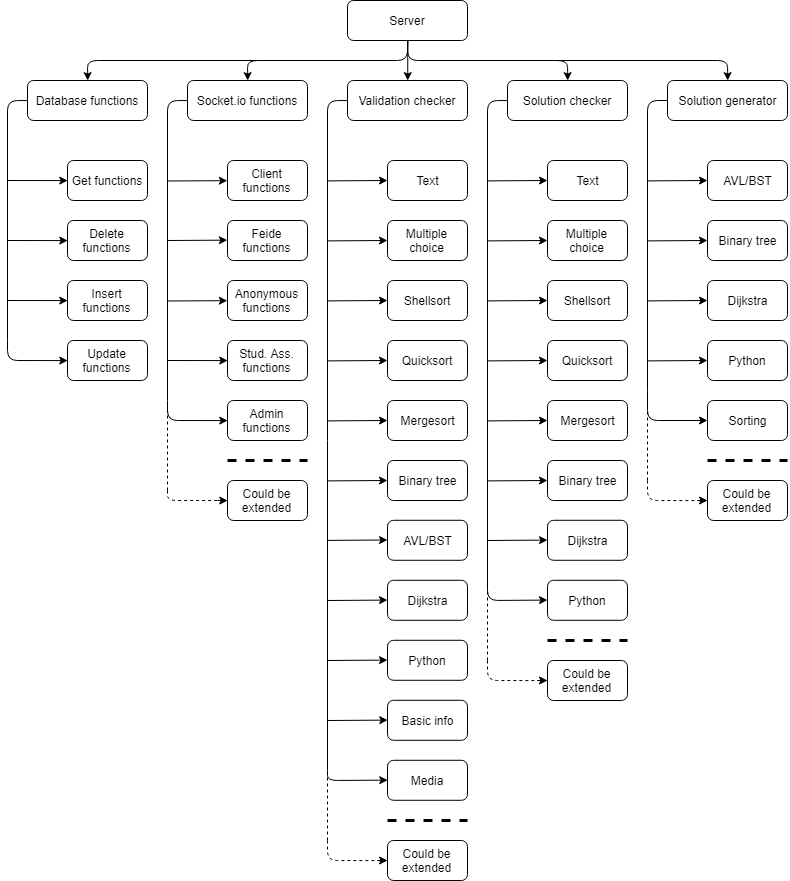
\includegraphics[width=\linewidth]{diagrammer/serverStructure}
    \caption{This is a diagram displaying the server structure and how the code is divided up into different subfiles}
    \label{fig:serverStructure}
\end{figure}